\chapter{Supramolecular Interactions of Group VI Metal Carbonyl Complexes: the Facilitating Role of 1,3-bis(\textit{p}-isocyanophenyl)urea}
\label{chap:supra}

The following chapter was published in Inorganic Chemistry in 2019 under authors Shaun Millard, Jenny W. Fothergill, Zoe Anderson, Dr. Eric C. Brown, Dr. Matthew D. King, and Dr. Adam C. Colson. My contributions to this paper were DFT calculations under the guidance of Dr. King.

\section{Abstract}

An investigation of supramolecular phenomena involving zero valent transition metal complexes was facilitated by the production of the ditopic isocyanide ligand 1,3-bis(\textit{p}-isocyanophenyl)urea, which was synthesized \textit{via} sub-stoichiometric phosgenation of 4-isocyanophenylamine and used to coordinate Group VI metal carbonyl fragments. The resulting binuclear organometallic complexes were observed to pack into ladder-like anisotropic arrays in the solid state. Crystallographic and computational evidence suggests that this packing motif can be attributed to a combination of intermolecular $\pi$-$\pi$ and urea-$\pi$ interactions. Similar to other \textit{N,N'}-diarylureas bearing electron withdrawing groups, 1,3-bis(\textit{p}-isocyanophenyl)urea and the organometallic complexes prepared therefrom also exhibit an affinity towards anion binding in non-aqueous solution. Equilibrium constants ($K$) for the formation of host-guest complexes between the organometallic derivatives of 1,3-bis(\textit{p}-isocyanophenyl)urea and chloride, nitrate, and acetate anions exceed $10^{3}$, $10^{4}$, and $10^{5}$ M$^{-1}$, respectively.   

\section{Introduction}

Non-covalent interactions are foundational to the field of supramolecular chemistry and have enabled emerging applications in chemical sensing, molecular recognition, and the self assembly of hierarchal materials \citep{Varshey2012, Schneider2009, Gale2012}. Such interactions are also exploited in the field of crystal engineering to direct the organization of molecular solids in which constituent molecules are arrayed according to desired structural motifs \citep{Desiraju2007a, Desiraju2013a, Mukherjee2015a, Corpinot2019a}. Although research efforts in these fields often emphasize the assembly of purely organic molecules, the integration of organometallic and coordination complexes into supramolecular structures and engineered molecular solids is also well-documented \citep{Chakrabarty2011, Cook2013a, Datta2018, Tanaka2014, Braga2017}. Less common, however, are accounts of supramolecular phenomena or crystal engineering involving low- or zero-valent transition metal carbonyl complexes, despite the fact that such complexes have long attracted interest due to their unique structural and electronic properties as well as the convenient spectroscopic monitoring afforded by the metal-bound carbon monoxide ligands \citep{Zukerman-Schpector2011, Chang2012a, Ramdass2013a, Ion2007, Coco2009, Karthikeyan2015, Thimmappa1995, Longoni1999}.

One challenge associated with the study of supramolecular behavior in low-valent transition metal complexes is the incorporation of organic ligands capable of binding to the electron-rich metal centers while simultaneously participating in non-covalent intermolecular interactions. To address this challenge, we have designed a ditopic organic ligand (\textbf{1}) bearing isocyanide functional groups appended to the well known \textit{N,N'}-diarylurea moiety (\autoref{dpu-structure}). Organic isocyanides are isolobal analogues of carbon monoxide and their ability to stabilize neutral and anionic transition metal complexes has been broadly demonstrated \citep{Sarapu1972, King1974, Cotton1960, Sarapu1975, Yamamoto1980, Weber1998, Leach1994, Warnock1989}. Unlike carbon monoxide, additional functionality can be conferred upon isocyanides by modification of the appended organic component, a useful feature that has been exploited in the preparation of chelating ligands, coordination polymers, and functional components in advanced materials \citep{Carpenter2016, Hahn1994, Hahn1992, Hahn1992b, Wagner2000, Carson2007, Tannenbaum1994, Carpenter2015a, Angelici2008, Horswell1999}.

\begin{figure}[h!]
    \centering
    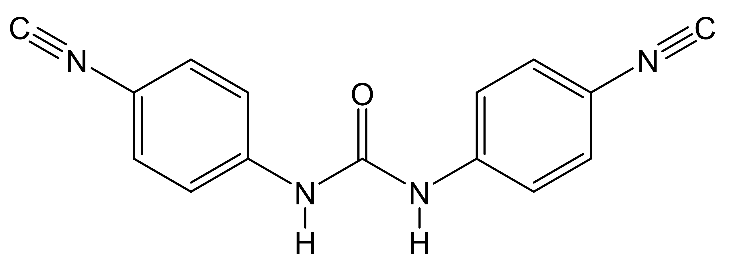
\includegraphics[width=0.8\linewidth]{figures/pub2/dpu-structure.png}
    \caption{1,3-bis(\textit{p}-isocyanophenyl)urea (\textbf{1})}\label{dpu-structure}
\end{figure}

Our selection of the \textit{N,N'}-diarylurea moiety as a facilitating agent for supramolecular chemistry and crystal engineering was motivated by the versatility of the urea group in promoting multiple intermolecular interactions  \citep{Schneider2009, Custelcean2008, Volz2011, Fischer2010, Pulka-Ziach2017}.
Examples of three prominent supramolecular motifs associated with the \textit{N,N'}-diarylurea moiety are depicted in \autoref{dpu-motifs}. 
The most intuitive non-covalent interactions are those between the N-H hydrogen bond donors and C=O acceptors of the urea group. 
In the absence of competing donor or acceptor species, these interactions can drive the formation of ribbon- or tape-like supramolecular structures (\autoref{dpu-motifs}a)\citep{Custelcean2008}. 
In the presence of alternative hydrogen bond acceptors such as halides or oxoanions, strong interactions are often observed between the urea host and the anionic guest (\autoref{dpu-motifs}b), presenting opportunities for applications in anion detection or anion-templated supramolecular assembly \citep{Custelcean2008, BlazekBregovic2015, Li2010d, Pfeifer2016, Boiocchi2004, Amendola2013, Esteban-Gomez2005, Amendola2010, Custelcean2006, Evans2014, Gale2011, Busschaert2015, Custelcean2010}. 
Perhaps less intuitively, the urea group is also known to facilitate $\pi$-$\pi$ interactions between neighboring \textit{N,N'}-diarylurea subunits (\autoref{dpu-motifs}c). 
The relative co-planarity of the aryl groups in \textit{N,N'}-diarylurea compounds is largely determined by the extent of intramolecular hydrogen bonding between the oxygen atom of the urea moiety and the \textit{ortho} proton located on the adjacent \textit{N}-aryl ring; experimental and computational evidence indicates that this planarity is most pronounced when the aryl rings bear electron withdrawing functional groups \citep{Custelcean2006, Reddy2007, Etter1990a, Etter1990, Etter1988a}.

\begin{figure}[h!]
    \centering
    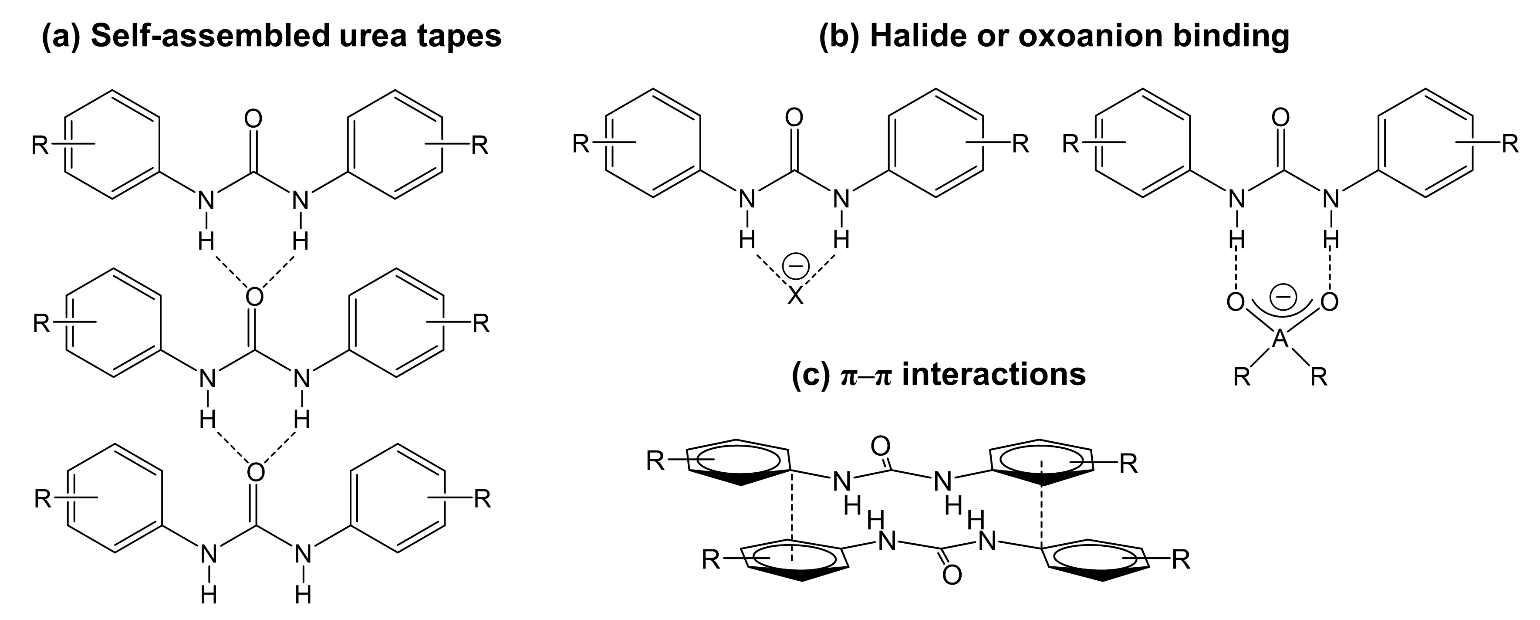
\includegraphics[width=0.8\linewidth]{figures/pub2/dpu-motifs.png}
    \caption{Major supramolecular motifs associated with \textit{N,N'}-diarylurea compounds}\label{dpu-motifs}
\end{figure}

The objective of the present study was to identify which---if any---of the supramolecular motifs depicted in \autoref{dpu-motifs} might be observed in \textit{N,N'}-diarylureas appended with zero-valent metal carbonyl subunits. Accordingly, we describe the synthesis of 1,3-bis(\textit{p}-isocyanophenyl)urea and its subsequent coordination to M(CO)$_{5}$ (M = Cr, Mo, and W) metal carbonyl fragments. A notable structural feature of these complexes is the nearly planar conformation of the \textit{N,N'}-diarylurea moiety, which facilitates molecular packing into ordered stacks through a combination of $\pi$-$\pi$ and urea-$\pi$ interactions. Like their purely organic counterparts, the metal bound derivatives of 1,3-bis(\textit{p}-isocyanophenyl)urea also exhibit an affinity towards anion binding in acetonitrile solution.

\section{Results and Discussion}

The ditopic 1,3-bis(\textit{p}-isocyanophenyl)urea ligand (\textbf{1}) was prepared by treating 4-isocyanophenylamine with a sub-stoichiometric quantity of triphosgene. The formation of \textbf{1} presumably proceeds through the intermediacy of an isocyanate species, although no attempts were made to isolate or characterize the latter \citep{Majer1994}. The PdO-catalyzed ligand substitution method described by \citet{Coville2015} was used to append Cr(CO)$_{5}$ and W(CO)$_{5}$ fragments to the isocyanide groups of \textbf{1}, producing homobimetallic complexes \textbf{2} and \textbf{4}, respectively. The Mo-containing variant (\textbf{3}) was prepared \textit{via} chemical decarbonylation of Mo(CO)$_{6}$ using trimethylamine \textit{N}-oxide in the presence of \textbf{1}. Complexes \textbf{2}, \textbf{3}, and \textbf{4} are readily identifiable by their diagnostic infrared spectra, as summarized in \autoref{tab:ir_freqs}. It is worth noting that the C$\equiv$N stretching frequency of \textbf{1} increases upon metal coordination, suggesting that the isocyanide acts primarily as a $\sigma$-donor with very little $\pi$-accepting character. This observation is consistent with previous reports of aromatic isocyanide coordination in heteroleptic metal carbonyls in which pronounced shifting of the C$\equiv$N stretch to lower frequencies was not observed until two or more isocyanide ligands were attached to a metal core \citep{Coville2015, Albers1982, Sattler2009}.

\begin{table}[]
\centering
\caption{Diagnostic infrared C$\equiv$N and C$\equiv$O stretching frequencies for compounds \textbf{1}-\textbf{4}.} \label{tab:ir_freqs}
\begin{tabular}{lll}
\multicolumn{3}{l}{\adjustimage{max size={0.9\linewidth}{0.9\paperheight}}{figures/pub2/dpu-sidegroups.png}}              \\ \hline
  & $\nu$ C$\equiv$N   (cm$^{-1}$) & $\nu$ C$\equiv$O (cm$^{-1}$) \\ \hline
1 & 2127           & N/A          \\
2 & 2143           & 2058, 1955   \\
3 & 2143           & 2063, 1956   \\
4 & 2144           & 2059, 1950   \\ \hline
\multicolumn{3}{l}{*Recorded in CH$_{2}$Cl$_{2}$}   
\end{tabular}
\end{table}

Single crystals of complexes \textbf{2}, \textbf{3}, and \textbf{4} suitable for X-ray diffraction studies were grown from acetonitrile solutions at -20 °C. As a representative example of the series, the molecular structure of \textbf{3} is shown in \autoref{complex3}. The most prominent structural feature is the nearly planar configuration of the \textit{N,N'}-diarylurea moiety. The C$_{ortho}$-C$_{ipso}$-N$_{urea-}$C$_{urea}$ torsion angles of 0.46° and 7.5° are similar to those reported by \citet{Reddy2007} for other \textit{N,N'}-diarylureas bearing para-substituted electron withdrawing groups. This planarity may be attributed to intermolecular C-H$\cdot \cdot \cdot$O hydrogen bonding between ortho aryl protons and the urea oxygen atom, as proposed by \citet{Etter1990a}; indeed, the C$_{ortho}\cdot \cdot \cdot$ O$_{urea}$ distances and C$_{ortho}$-H$\cdot \cdot \cdot$ O$_{urea}$ angles in complexes \textbf{2}, \textbf{3}, and \textbf{4} range from 2.84 to 2.87 \AA~ and 121 to 122°, respectively, and are consistent with the analogous distances (2.83 to 2.94 \AA~) and angles (119 to 122°) observed in other \textit{N,N'}-diarylureas of comparable planarity \citep{Reddy2007, Etter1990a}. Salient structural features for complexes \textbf{2} and \textbf{4} are presented in \autoref{tab:measurements} and \autoref{fig:complex2} and \autoref{fig:complex4} in the Supporting Information. 

\begin{figure}[h!]
    \centering
    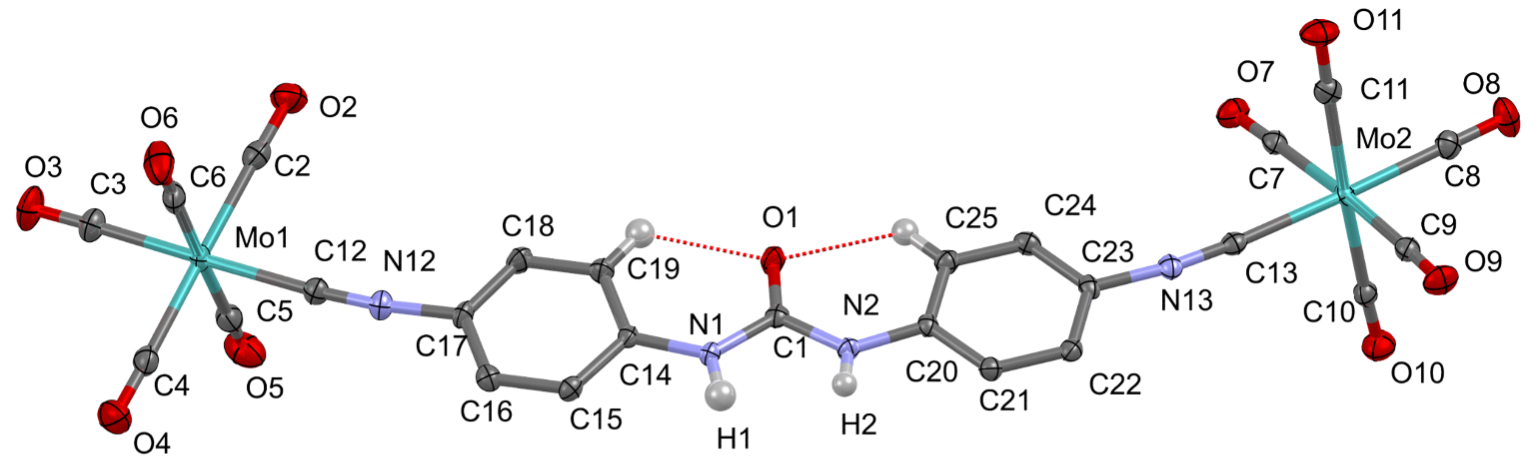
\includegraphics[width=0.8\linewidth]{figures/pub2/complex3.png}
    \caption{Molecular structure of complex \textbf{3}. Thermal ellipsoids are rendered at the 50\% probability level. Only urea N-H atoms and aromatic hydrogen atoms participating in hydrogen bonding are shown.}\label{complex3}
\end{figure}

\begin{table}[]
\centering
\caption{Selected bond distances, close contacts, and torsion angles for complexes \textbf{2}, \textbf{3}, and \textbf{4}} \label{tab:measurements}
\begin{tabular}{llll}
\hline
 & \textbf{2} (M = Cr) & \textbf{3} (M = Mo) & \textbf{4} (M = W) \\ \hline
 & \multicolumn{3}{c}{\rule{0pt}{3ex} \textbf{Distances (\AA)}} \\
M - C$_{isocyanide}$ & \multicolumn{1}{l|}{1.981(2), 1.979(2)} & \multicolumn{1}{l|}{2.127(2), 2.130(2)} & 2.119(3), 2.113(3) \\
C$_{ortho}$ - H$\cdot \cdot \cdot$O$_{urea}$ & \multicolumn{1}{l|}{2.24, 2.22} & \multicolumn{1}{l|}{2.25, 2.23} & 2.25, 2.23 \\
C$_{ortho}\cdot \cdot \cdot$O$_{urea}$ & \multicolumn{1}{l|}{2.86, 2.84} & \multicolumn{1}{l|}{2.86, 2.84} & 2.87, 2.84 \\
$\pi$-$\pi$ contacts \ddag & \multicolumn{1}{l|}{3.31} & \multicolumn{1}{l|}{3.33} & 3.32 \\
urea-$\pi$ contacts \ddag & \multicolumn{1}{l|}{3.29} & \multicolumn{1}{l|}{3.32} & 3.31 \\
 & \multicolumn{3}{c}{\rule{0pt}{3ex} \textbf{Angles (°)}} \\
C$_{ortho}$-H$\cdot \cdot \cdot$O$_{urea}$ & \multicolumn{1}{l|}{121.8, 121.3} & \multicolumn{1}{l|}{121.8. 121.0} & 121.0, 122.0 \\
C$_{ortho}$-C$_{ipso}$-N$_{urea}$-C$_{urea}$ & \multicolumn{1}{l|}{1.1, 6.1} & \multicolumn{1}{l|}{0.46, 7.5} & 0.45, 7.8 \\ \hline
\multicolumn{4}{l}{\ddag distance between adjacent mean \textit{N,N'}‑diarylurea molecular planes} 
\end{tabular}
\end{table}

The packing of \textbf{3} within the molecular solid is depicted in \autoref{molecular-packing}a. Despite the relative steric bulk of the Mo(CO)$_{5}$ subunits, the planarity of the \textit{N,N'}-diarylurea moiety facilitates packing into ordered stacks, resulting in staggered, ladder-like arrays of metal atoms (\autoref{molecular-packing}b). It is tempting to view the orientation and proximity of these metal sites and speculate on the potential development of charge transfer materials, especially considering that adjacent metal atoms are separated by only 6.0 to 7.6 \AA. This separation is well within the 4 to 14 \AA~ range over which the majority of electron transfer processes occur in benchmark biological systems \citep{Page1999a, Moser2006}. In their present form, however, complexes \textbf{2}, \textbf{3}, and \textbf{4} undergo electrochemically irreversible oxidation and are therefore unlikely candidates for such applications (\autoref{fig:cv}). 

\begin{figure}[h!]
    \centering
    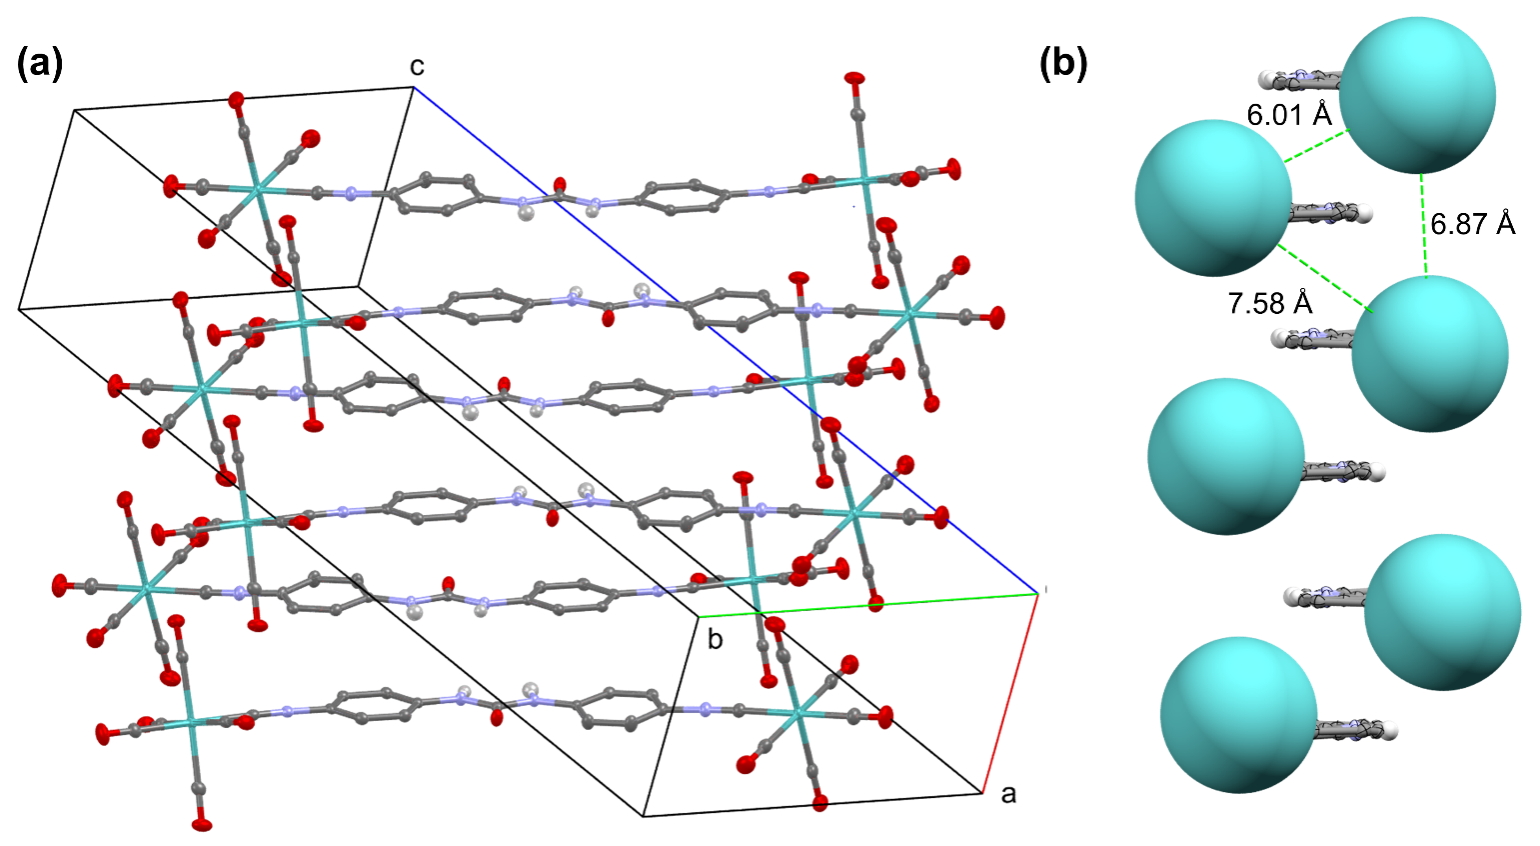
\includegraphics[width=0.8\linewidth]{figures/pub2/molecular-packing.png}
    \caption{\textbf{(a)} Molecular packing of \textbf{3} showing the orientation of the molecules relative to the unit cell axes. \textbf{(b)} Alternative representation of the molecular packing of  \textbf{3} viewed through the \textit{N,N'}-diarylurea planes with the CO ligands omitted and Mo atoms depicted at full Van der Waals radius.}\label{molecular-packing}
\end{figure}

The molecular packing of \textbf{3} is reminiscent of the $\pi$-stacking motif introduced in \autoref{dpu-motifs}c in which planar \textit{N,N'}-diarylurea moieties are arranged parallel to one another in an offset or “slipped” orientation; however, close inspection of the interactions between molecules of \textbf{3} reveals several subtle deviations from the archetypal packing motif. As shown in \autoref{stacking}a, the separation between the adjacent \textit{N,N'}-diarylurea planes of complex \textbf{3} is $\sim$3.32 \AA, while the distance between the centroids of interacting aromatic rings alternates between 3.76 and 4.79 \AA. By comparison, previous structural studies of \textit{N,N'}-diarylureas bearing electron withdrawing functional groups have reported interplanar distances of 3.4 to 3.5 \AA, with the aromatic centroids separated by no more than 4.2 \AA~ \citep{Reddy2007, Solomos2017a} Although the interplanar distances associated with complex \textbf{3} are consistent with other $\pi$-$\pi$ interactions reported in the literature, the significant separation between alternating pairs of ring centroids suggest that $\pi$-$\pi$ interactions are not the only non-covalent interactions contributing to the close contact between \textit{N,N'}-diarylurea planes \cite{Janiak2000}. Additional insight into the nature of a secondary interaction can be gained by viewing adjacent pairs of \textit{N,N'}-diarylurea moieties from a direction normal to the molecular planes (\autoref{stacking}b). From this perspective, it becomes apparent that the interactions between an arbitrary \textit{N,N'}-diarylurea moiety of complex \textbf{3} and the molecules positioned directly above and below are not equivalent---one face of the aromatic ring experiences substantial overlap with the \textit{aromatic ring} of a neighboring molecule, while the opposite face interacts with the \textit{nitrogen atom} of a different neighbor. In the latter case, the distance between the aromatic ring centroid and the urea nitrogen atom is only 3.34 \AA, suggesting the existence of a non-covalent urea-$\pi$ interaction. Similar close contacts are also observed in the Cr- and W-containing derivatives (\textbf{2} and \textbf{4}), as tabulated in \autoref{tab:measurements}.

\begin{figure}[h!]
    \centering
    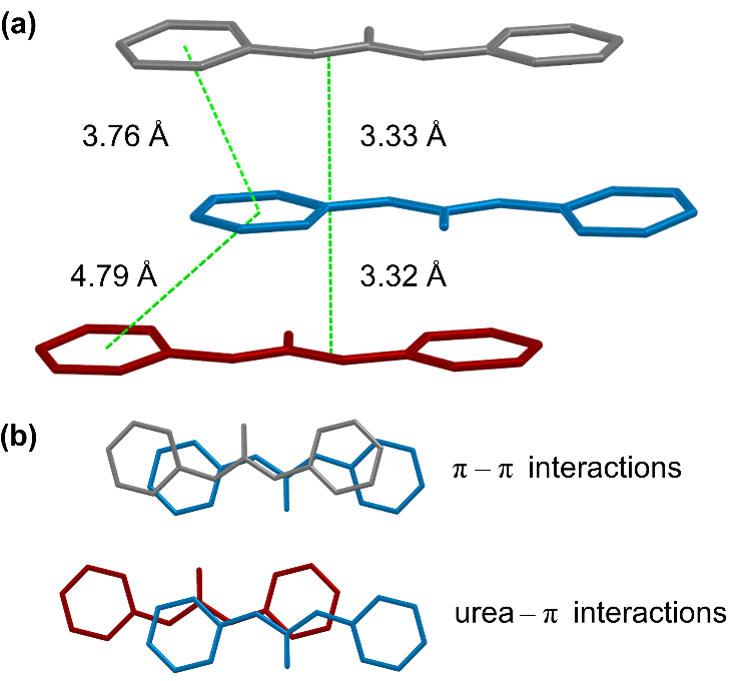
\includegraphics[width=0.8\linewidth]{figures/pub2/stacking.png}
    \caption{\textbf{(a)} Distances between adjacent \textit{N,N'}-diarylurea planes and the aromatic ring centroids of complex \textbf{3}. \textbf{(b)} Alternating stacking motifs viewed normal to the \textit{N,N'}-diarylurea planes. Hydrogen atoms and all ring substituents are omitted for clarity.}\label{stacking}
\end{figure}

Interactions between aromatic $\pi$-systems and urea or amide moieties have been predicted computationally and observed experimentally, although reports of such interactions outside of a biological context are scarce \citep{Imai2009, Kasavajhala2015, Goyal2017a, Ema2018}. Because urea-$\pi$ interactions are not commonly observed in synthetic systems, computational methods were employed to determine whether urea-$\pi$ interactions truly contribute to the molecular packing observed for complexes \textbf{2}, \textbf{3}, and \textbf{4}, or if the packing motif is simply an artifact of the steric encumbrance imposed by the Mo(CO)$_{5}$ groups. 

Initial solid-state DFT calculations were performed on the crystal structure of complex \textbf{3} to assess lattice energy in terms of cohesive and conformational strain energies associated with crystal packing. The basis set superposition error-corrected lattice energy was determined to be -123.20 kcal mol$^{-1}$, which accounts for the balance of -172.86 kcal mol$^{-1}$ of cohesive energy offset with 49.65 kcal mol$^{-1}$ of adverse molecular strain energy due to deformations emerging from crystal packing forces (\autoref{tab:3-energies}). This significant contribution of molecular strain to the overall lattice energy, primarily in the \textit{N,N'}-diarylurea moieties, likely results from steric effects of geometric packing of the bulky Mo(CO)$_{5}$ end groups. 

\begin{table}[]
\centering
\caption{Calculated energies per molecule (kcal mol$^{-1}$) of complex \textbf{3} in the crystal and dimer conformations.} \label{tab:3-energies}
\begin{tabular}{lll}
\multicolumn{3}{c}{\textbf{Complex 3}} \\ \hline
\multicolumn{2}{l}{Total Lattice Energy} & -123.20 \\
\multicolumn{2}{l}{~~~~Cohesive Energy} & -172.86 \\
\multicolumn{2}{l}{~~~~Conformational Energy} & 49.65 \\
\multicolumn{3}{c}{\rule{0pt}{5ex} \textbf{Complex 3 Dimers}} \\ \hline
 & $\pi$ - $\pi$ & urea - $\pi$ \\
Total Binding Energy & -118.43 & -111.64 \\
Relative Binding Energy & 0.000 & 6.797 \\
\multicolumn{3}{c}{\rule{0pt}{5ex} \textbf{\textit{N,N'}‑diarylurea Dimers}} \\ \hline
 & $\pi$ - $\pi$ & urea - $\pi$ \\
Total Binding Energy & -57.92 & -55.62 \\
Relative Binding Energy & 0.000 & 2.295 \\ \hline
\end{tabular}
\end{table}

To allocate the relative contributions of the substituent $\pi$-$\pi$ and urea-$\pi$ stacking motifs described in \autoref{stacking} to the complex \textbf{3} lattice energy, appropriate dimer configurations were isolated from the DFT-optimized solid-state structure. Single-point energy calculations were performed to obtain dimer and single-molecule energies for the models representative of their strained solid-state molecular conformations. It was found that the two motifs are comparable in interaction energy, with total binding energies of -118.43 and -111.64 kcal mol$^{-1}$ for the $\pi$-$\pi$ and urea-$\pi$ stacking motifs, respectively, corresponding to a $\Delta E_{bind}$  of only 6.80 kcal mol$^{-1}$ favoring the $\pi$-$\pi$ intermolecular interactions. These stacked dimer models, however, still contained interacting Mo(CO)$_{5}$ end groups, thereby not adequately representing the true nature or relative consequence of the two participating \textit{N,N'}-diarylurea stacking motifs.

 Subsequent calculations isolated the interaction energy contributions to the \textit{N,N'}-diarylurea $\pi$-$\pi$ and urea-$\pi$ stacking motifs, for which the Mo(CO)$_{5}$ groups were removed from the molecular models. The \textit{p}-substituent isocyanides groups were terminated with H atoms to provide a better representation of the bonding configuration of the \textit{N,N'}-diarylurea moieties as they exist in the complex \textbf{3} crystal structure. The resulting calculations produced absolute \textit{N,N'}-diarylurea dimer interaction energies of -57.92 and -55.62 kcal mol$^{-1}$, respectively. Remarkably, this amounts to an approximate difference of only 4\% (\textit{i.e.} 2.30 kcal mol$^{-1}$) between the $\pi$-$\pi$ and urea-$\pi$ stacking interactions of the \textit{N,N'}-diarylurea groups, despite the reduction of surface contact area from 94.8 to 76.4 \AA \citep{Desiraju2007a, Desiraju2013a, Mukherjee2015a, Corpinot2019a} for the urea-$\pi$ stacked dimer (based on MSMS surface area calculated using 1.5-\AA~ probe sphere). These results demonstrate that the urea-$\pi$ stacking is indeed a robust intermolecular interaction and plays an important role in molecular ordering during crystal growth, and that the association is not an ancillary product of crystal packing.
 
The underlying nature of the prominent urea-$\pi$ stacking interactions observed in the synthetic complexes can be explained through observation of electrostatic potentials and molecular orbital interactions. An electrostatic potential map of the urea-$\pi$ stacked \textit{N,N'}-diarylurea dimer shows that the positive electrostatic potential arising from the urea nitrogen atom overlaps with the negative potential central to an aromatic ring of the adjacent molecule (\autoref{esp-surface}). The proximity of the molecules in the urea-$\pi$ dimer pair, separated by 3.32 \AA, provides a favorable distance for strong electrostatic interaction between these substituent groups. In addition, inspection of molecular orbitals reveals that the \textit{N,N'}-diarylurea HOMO and LUMO share significant constructive spatial overlap in their relative dimer positions (\autoref{mo-surface}). The individual molecule orbital energies were calculated at -6.344 and -1.601 eV for the HOMO and LUMO, respectively. The resulting HOMO of the dimer complex, representative of the single-molecule orbital combination formed in the crystalline orbital, was calculated at -6.439 eV. The combination of advantageous electrostatic interactions and molecular orbital interactions provides the physical description for the strong interaction evident in the urea-$\pi$ stacking of the \textit{N,N'}-diarylurea dimer in the crystal structure of complex \textbf{3}. 

\begin{figure}[h!]
    \centering
    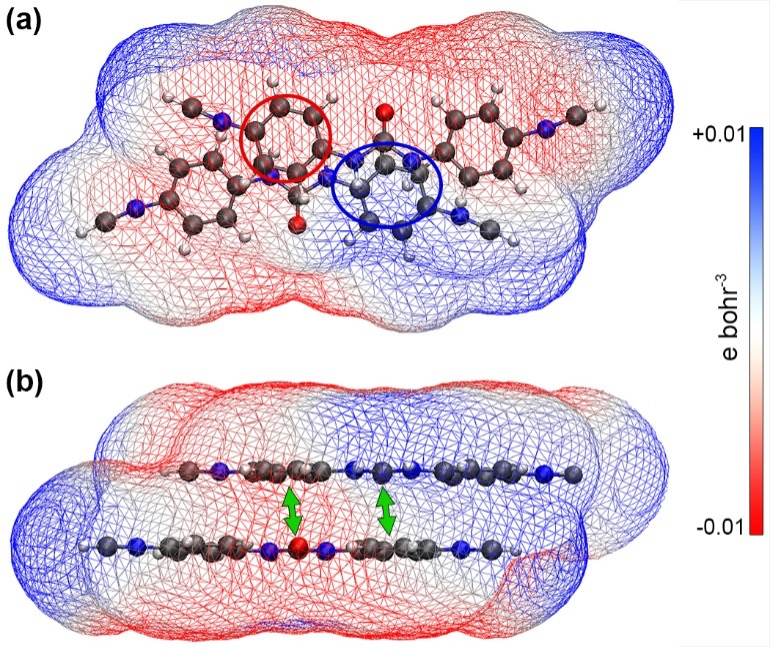
\includegraphics[width=0.8\linewidth]{figures/pub2/esp-surface.jpg}
    \caption{Electrostatic potentials mapped onto the electron density isosurface (isovalue: 1.0 × 10$^{-6}$ \textit{e} bohr$^{-3}$) of the \textit{N,N'}-diarylurea urea-$\pi$ stacked dimer. \textbf{(a)} Top view of urea-$\pi$ dimer indicating urea nitrogen atoms (blue circle) and the aromatic ring (red circle) of the upper molecule involved in electrostatic binding interactions. \textbf{(b)} Locations of the two nitrogen-ring interactions (green arrows) in the \textit{N,N'}-diarylurea urea-$\pi$ dimer.}\label{esp-surface}
\end{figure}

\begin{figure}[h!]
    \centering
    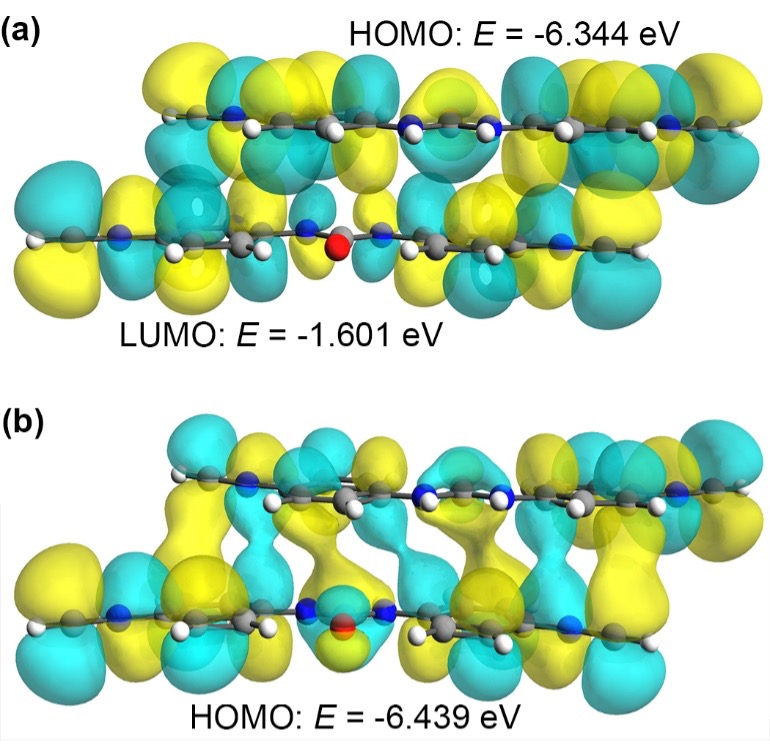
\includegraphics[width=0.8\linewidth]{figures/pub2/mo-surface.jpg}
    \caption{Molecular orbital surface representations of \textit{N,N'}-diarylurea \textbf{(a)} HOMO and LUMO orbitals for non-interacting molecules in the urea-$\pi$ stacked dimer orientation, and \textbf{(b)} the resulting HOMO of the \textit{N,N'}-diarylurea urea-$\pi$ dimer.}\label{mo-surface}
\end{figure}

Having investigated the intermolecular interactions between complexes \textbf{2}-\textbf{4} in the solid state, a short study of the anion-binding behavior of \textbf{1}-\textbf{4} in non-aqueous solution was initiated. Urea containing compounds are known to act as effective receptors or hosts for anionic guests \citep{Custelcean2008, BlazekBregovic2015, Li2010d, Pfeifer2016, Boiocchi2004, Amendola2013, Esteban-Gomez2005, Amendola2010, Custelcean2006, Evans2014, Gale2011, Busschaert2015, Custelcean2010}. The host-guest interaction of interest can be represented by the following equilibrium relationship: $host + guest^{-} \rightleftharpoons [host\cdot guest]^{-}$. The corresponding equilibrium constant ($K$) may be estimated by performing spectroscopic titration experiments followed by fitting of the resultant data to established binding models \cite{Thordarson2011, BrynnHibbert2016}. In the present study, solutions of \textbf{1}-\textbf{4} were titrated with the tetrabutylammonium salts of chloride, nitrate, and acetate as representative examples of the halides, inorganic oxoanions, and organic oxoanions, respectively. 

$^{1}$H NMR spectroscopy was selected as the primary method for estimating equilibrium binding constants, as incremental titration of urea hosts 1-4 with anionic guests consistently produced a detectable response in the spectral features. Under the dilute conditions of the titration experiments ($\approx$ 0.1 mM), broadening of the urea N-H proton NMR signals prevented unambiguous chemical shift assignment. Consequently, the $^{1}$H NMR signals corresponding to the aromatic ring protons were used to probe anion binding behavior. Two unique aromatic proton resonances were observed for compounds 1-4, a downfield signal corresponding to the pair of protons nearest the urea moiety (H$_{\alpha}$) and an upfield signal representing the pair of protons nearest the isocyanide functional group (H$_{\beta}$). The latter signal shifts upfield upon titration and was used to determine K for all host-guest complexes, as the former signal (H$_{\alpha}$) was prone to considerable broadening, especially during titrations with acetate. 
As a representative example, \autoref{HNMR} a illustrates the effects of chloride titration on the aromatic $^{1}$H NMR signals of \textbf{1}, while \autoref{HNMR} b compares the magnitude of the $^{1}$H NMR chemical shifts of H$_{\beta}$ observed upon titration of \textbf{1} with nitrate, chloride, and acetate anions.    

\begin{figure}[h!]
    \centering
    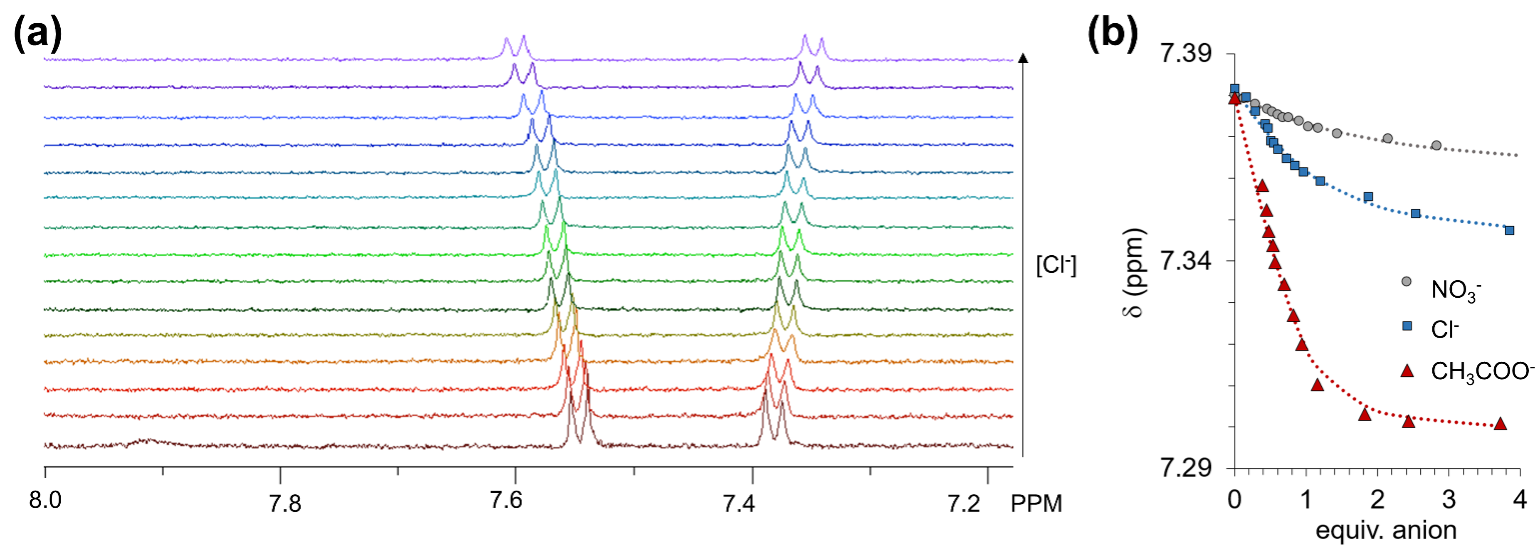
\includegraphics[width=0.8\linewidth]{figures/pub2/HNMR.png}
    \caption{\textbf{(a)} Overlay of $^{1}$H NMR spectra obtained during the titration of \textbf{1} (0.90 x 10$^{-4}$ M in CD$_{3}$CN) with [Bu$_{4}$N]Cl. \textbf{(b)} Comparison of $^{1}$H NMR chemical shifting observed during titration of  \textbf{1} with nitrate, chloride, and acetate anions. The dotted lines represent the results of non-linear fitting to a 1:1 host-guest binding model.}\label{HNMR}
\end{figure}

The respective upfield and downfield shifts observed for the H$_{\beta}$ and H$_{\alpha}$ $^{1}$H NMR signals are consistent with previous observations of signal shifting during titration of \textit{N,N'}-diarylureas with anions \citep{Boiocchi2004, Smith1992, Regueiro-Figueroa2010, Clare2009}. It should be noted that deprotonation of \textit{N,N'}-diarylureas has been reported during titrations with basic anions such as fluoride or acetate, especially when the urea (or thiourea) hosts are particularly acidic \citep{Amendola2010, Carreira-Barral2017}. As a means of confirming that the observed $^{1}$H NMR chemical shifts may be attributed to host-guest complex formation rather than deprotonation of the \textit{N,N'}-diarylurea host, UV-Vis spectroscopy was used to probe the magnitude of the bathochromic spectral shift accompanying addition of excess acetate anion. Formation of hydrogen bonding host-guest complexes is typically characterized by a modest spectral shift (< 50 nm), while formal deprotonation produces an absorption band that is generally red-shifted by more than 100 nm \citep{Boiocchi2004, Esteban-Gomez2005, Gomez2005}. Addition of excess acetate to  \textbf{1} produced a bathochromic spectral shift of only 15 nm with no additional features appearing at higher wavelengths, indicating that the urea moiety remains protonated under the titration conditions (\autoref{fig:uvvis}).     

Equilibrium constants for the formation of host-guest complexes of \textbf{1}-\textbf{4} with chloride, nitrate, and acetate were derived from $^{1}$H NMR titration profiles and are reported in \autoref{tab:eq_constants}. All values of $K$ assume a 1:1 binding ratio between the urea host and anion guest, an assumption substantiated by direct observation of the 1:1 host-guest complexes using electrospray ionization mass spectrometry as well as the consistency of the 1:1 binding model in accounting for the experimental data (\autoref{fig:esi1}-\autoref{fig:hnmr-shift})\citep{Thordarson2011}. Compounds \textbf{1}-\textbf{4} exhibit similar affinities for each of the anions studied, the values of $K$ becoming progressively larger with increasing anion basicity. The equilibrium constants for the formation of host-guest complexes of \textbf{1}-\textbf{4} with chloride and nitrate anions are comparable to those reported by \citet{Boiocchi2004} for the 1,3-bis(\textit{p}-nitrophenyl)urea receptor, although a higher affinity towards acetate was measured for the latter (log $K$ = 6.61). The results presented in \autoref{tab:eq_constants} suggest that the isocyanide functionalized \textit{N,N'}-diarylurea (\textbf{1}) is capable of strong anion-binding and that attachment of organometallic subunits does not substantially impact the ability of the urea moiety to act as an anion receptor. 

\begin{table}[]
\centering
\caption{Equilibrium constants (log $K$) for formation of host-guest complexes of \textbf{1}-\textbf{4} with selected anions} \label{tab:eq_constants}
\begin{tabular}{llll}
 & \multicolumn{3}{c}{log $K^{a}$} \\ \hline
\rule{0pt}{2ex} Urea Host & NO$_{3}^{-}$ & Cl$^{-}$ & CH$_{3}$COO$^{-}$ \\ \hline
1 & 3.62(5) & 4.42(3) & 5.30(8) \\
2 & 3.52(3) & 4.35(3) & 5.41(7) \\
3 & 3.60(3) & 4.35(8) & 5.50(3) \\
4 & 3.70(3) & 4.58(3) & 5.66(4) \\ \hline
\multicolumn{4}{l}{\makecell[l]{$^{a}$ In CD$_{3}$CN solution at 25 °C. Values in \\parentheses indicate uncertainty in the \\ last figure}}
\end{tabular}
\end{table}

\section{Conclusions}

The synthesis of 1,3-bis(\textit{p}-isocyanophenyl)urea, its coordination to Group VI metal carbonyl fragments, and the structural characterization of the binuclear organometallic products have been reported. The nearly planar configuration of the \textit{N,N'}-diarylurea moiety enables the packing of the organometallic complexes into ladder like anisotropic arrays in which the zero valent metal atoms are separated by 6.0 to 7.6 \AA. Crystallographic and computational evidence suggests that that the formation of these arrays can be attributed to a combination of intermolecular $\pi$-$\pi$ and urea-$\pi$ interactions. Although the metal carbonyl fragments employed in this exploratory study undergo irreversible electrochemical oxidation, the methods and observations reported herein might be extended to produce similar molecular solids containing more electrochemically-robust organometallic fragments; specimens of the latter may in turn find application as charge transfer materials. Similar to other \textit{N,N'}-diarylureas bearing electron withdrawing groups, 1,3-bis(\textit{p}-isocyanophenyl)urea and its organometallic derivatives were also found to behave as anion receptors in non-aqueous solvent. Equilibrium constants ($K$) for the formation of host-guest complexes of 1,3-bis(\textit{p}-isocyanophenyl)urea with chloride, nitrate, and acetate exceed 10$^{3}$, 10$^{4}$, and 10$^{5}$ M$^{-1}$, respectively. Complexes of 1,3-bis(\textit{p}-isocyanophenyl)urea with Group VI metal carbonyl complexes exhibit similar anion binding behaviors, presenting opportunities for additional research into anion detection or anion-templated supramolecular assembly using low-valent organometallic species.

\section{Experimental}
\subsection{General Considerations}
All synthetic operations were carried out under a nitrogen atmosphere using standard Schlenk techniques to exclude moisture and oxygen. Nitrogen was prepurified by passage through columns of activated copper catalyst (BASF PuriStar R3-11G) and molecular sieves (RCI-DRI 13X). Glassware was dried in an oven at 130 °C, assembled while hot, and allowed to cool under reduced pressure. All solvents were dried according to published procedures and degassed with nitrogen prior to use.21 Cr(CO)$_{6}$ (Beantown Chemical, 99\%), Mo(CO)$_{6}$ (Acros, 98\%), W(CO)$_{6}$ (Beantown Chemical, 97\%), PdO (Acros), trimethylamine \textit{N}-oxide dihydrate (Beantown Chemical, 98\%), and triphosgene (Chem Impex, 99\%) were used as received without further purification. 4-Isocyanophenylamine was prepared according to literature procedures and sublimed prior to use \citep{Heinze2003}. 

Infrared spectra were obtained using a Thermo Scientific Nicolet iS5 FTIR spectrometer equipped with a 0.2 mm BaF$_{2}$ liquid cell. $^{1}$H and $^{13}$C NMR data were recorded on a 600 MHz Bruker AVANCE III spectrometer. Electrospray ionization mass spectrometry (ESI-MS) was carried out using a Bruker HCTultra CTD II spectrometer in negative ion mode. Samples of \textbf{1}-\textbf{4} were dissolved in CH$_{3}$CN and treated with the tetrabutylammonium salts of chloride, nitrate, and acetate prior to injection into the mass spectrometer. Elemental analyses were performed by Atlantic Microlab, Inc in Norcross, GA, USA. 

\subsection{Synthesis of 1,3-bis(\textit{p}-isocyanophenyl)urea (\textbf{1})}
4-isocyanophenylamine (3.00 g, 25.4 mmol) was dissolved in 80 mL of anhydrous dichloromethane, followed by addition of 7.8 mL of triethylamine. The solution was cooled to 0 °C and triphosgene (1.20 g, 4.04 mmol) was slowly introduced into the reaction vessel. (\textit{CAUTION: Triphosgene is toxic and its reaction with 4-isocyanophenylamine generates considerable heat and an abundance of hydrogen chloride. Triphosgene should be added very slowly and in several portions to allow for sufficient heat exchange with the cooling media.}) The light yellow reaction mixture was magnetically stirred for 3 hours at 0 °C, then stirred for an additional 45 hours at 25 °C. Methanol (10 mL) was added to the reaction mixture and stirring was continued for an additional hour.
Organic solvents were removed under reduced pressure, and the residues were dissolved in 60 mL of dimethyl formamide (DMF). Deionized water (60 mL) was slowly added, and the reaction vessel was gently heated to ensure that the solution remained clear. After addition of deionized water, the solution was allowed to cool slowly to room temperature, whereupon an off-white precipitate formed. The precipitate was filtered and washed with three 20 mL portions of water, followed by 20 mL of diethyl ether and 20 mL of hexanes, respectively. After drying under reduced pressure for one day,  \textbf{1} was obtained with sufficient purity for further experimentation. 
Yield: 2.82 g (84.6\%). IR (CH$_{2}$Cl$_{2}$, cm$^{-1}$): $\nu_{CN}$ 2027 (vs). 
$^{1}$H NMR (CD$_{3}$CN, 20 °C): $\delta$ 7.38 (d, 4H, Ar-\textit{H}, \textit{J} = 8.86), 7.53 (d, 4H, Ar-\textit{H}, \textit{J} = 8.86), 7.60 (br s, 2H, N-\textit{H}). $^{13}$C NMR (CD$_{3}$CN, 20 °C): $\delta$ 119.3, 127.1, 140.3, 151.9, 163.5, \textit{ipso C} not observed. MS(ESI): \textit{m/z} 297 [M + Cl$^{-}$]$^{-}$, 324 [M + NO3$^{-}$]$^{-}$, 321 [M + CH$_{3}$COO$^{-}$]$^{-}$. Anal. Calcd for C$_{15}$H$_{10}$N$_{4}$O: C, 68.69; H, 3.84; N, 21.36. Found: C, 68.47; H, 4.05; N, 21.17.            

\subsection{Synthesis of Complex \textbf{2}}
Cr(CO)$_{6}$ (317 mg, 1.44 mmol) and  \textbf{1} (182 mg, 0.694 mmol) were combined with 25 mL of DMF and heated to 90 °C, whereupon PdO (14 mg, 0.12 mmol) was added to the reaction vessel. The reaction mixture was magnetically stirred at 90 °C for 15 minutes, then allowed to cool to room temperature. DMF was removed by vacuum distillation, leaving behind an oily residue. The oily residue was extracted with dichloromethane and filtered to remove insoluble impurities. Hexanes were added slowly to the dichloromethane filtrate until the solution became cloudy, then the solution was centrifuged at 5000 rpm for 2 minutes, after which the clear supernatant was decanted and dried under reduced pressure. The residual pale yellow solid was dissolved in warm acetonitrile, then cooled slowly to -20 °C to yield crystals of \textbf{2} $\cdot$ CH$_{3}$CN. Yield: 242 mg (50.7\%). IR (CH$_{2}$Cl$_{2}$, cm$^{-1}$): $\nu_{CN}$ 2143 (m), $\nu_{CO}$ 2058 (s), 1955 (vs). $^{1}$H NMR (CD$_{3}$CN, 20 °C): $\delta$ 7.44 (d, 4H, Ar-\textit{H}, \textit{J} = 8.75), 7.58 (d, 4H, Ar-\textit{H}, \textit{J} = 8.89), 7.71 (br s, 2H, N-\textit{H}). $^{13}$C NMR (CD$_{3}$CN, 20 °C): $\delta$ 120.2, 127.9, 141.1, 153.0, isocyanide and adjacent \textit{ipso} carbons not observed. MS(ESI): \textit{m/z} 681 [M + Cl$^{-}$]$^{-}$, 708 [M + NO$_{3}^{-}$]$^{-}$, 705 [M + CH$_{3}$COO$^{-}$]$^{-}$. Anal. Calcd for C$_{27}$H$_{13}$Cr$_{2}$N$_{5}$O$_{11}$: C, 47.18; H, 1.91; N, 10.19. Found: C, 47.23; H, 1.83; N, 10.16.

\subsection{Synthesis of Complex \textbf{3}}
Mo(CO)$_{6}$ (811 mg, 3.07 mmol) and \textbf{1} (403 mg, 1.54 mmol) were dissolved in 25 mL of tetrahydrofuran (THF). A dropping funnel charged with trimethylamine N oxide dihydrate (342 mg, 3.07 mmol), THF (10 mL), and methanol (10 mL) was attached to the reaction flask, the contents of which were added dropwise to the reaction mixture over the course of 1 hour. The reaction mixture was magnetically stirred for 6 hours at room temperature, after which the solvents were removed under reduced pressure. The residues were extracted with dichloromethane and filtered to remove insoluble impurities. Hexanes were added slowly to the dichloromethane filtrate until the solution became cloudy, then the solution was centrifuged at 5000 rpm for 2 minutes, after which the clear supernatant was decanted and dried under reduced pressure. The residual off-white solid was dissolved in warm acetonitrile, then cooled slowly to  20 °C to yield crystals of \textbf{3}. Yield: 871 mg (77.0\%). IR (CH$_{2}$Cl$_{2}$, cm$^{-1}$): $\nu_{CN}$ 2143 (m), $\nu_{CO}$ 2063 (s), 1956 (vs). $^{1}$H NMR (CD$_{3}$CN, 20 °C): $\delta$ 7.43 (d, 4H, Ar-\textit{H}, \textit{J} = 8.86), 7.57 (d, 4H, Ar-\textit{H}, \textit{J} = 8.82), 7.69 (br s, 2H, N-\textit{H}). $^{13}$C NMR (CD$_{3}$CN, 20 °C): $\delta$ 119.3, 127.2, 140.4, 151.8, isocyanide and adjacent \textit{ipso} carbons not observed. MS(ESI): \textit{m/z} 769 [M + Cl$^{-}$]$^{-}$, 796 [M + NO$_{3}^{-}$]$^{-}$, 793 [M + CH$_{3}$COO$^{-}$]$^{-}$. Anal. Calcd for C$_{25}$H$_{10}$Mo$_{2}$N$_{4}$O$_{11}$: C, 40.89; H, 1.37; N, 7.63. Found: C, 41.03; H, 1.38; N, 8.15.

\subsection{Synthesis of Complex \textbf{4}}
W(CO)$_{6}$ (369 mg, 1.05 mmol) and \textbf{1} (132 mg, 0.503 mmol) were combined with 25 mL of DMF and heated to 90 °C, whereupon PdO (10 mg, 0.082 mmol) was added to the reaction vessel. The reaction mixture was magnetically stirred at 90 °C for 5 minutes, then cooled to room temperature. DMF was removed by vacuum distillation, leaving behind an oily residue. The oily residue was extracted with dichloromethane and filtered to remove insoluble impurities. Hexanes were added slowly to the dichloromethane filtrate until the solution became cloudy, then the solution was centrifuged at 5000 rpm for 2 minutes, after which the clear supernatant was decanted and dried under reduced pressure. The residual yellow solid was dissolved in warm acetonitrile, then cooled slowly to -20 °C to yield crystals of \textbf{4} $\cdot$ CH$_{3}$CN. Yield: 211 mg (44.1\%). IR (CH$_{2}$Cl$_{2}$, cm$^{-1}$): $\nu_{CN}$ 2144 (m), $\nu_{CO}$ 2059 (s), 1950 (vs). $^{1}$H NMR (CD$_{3}$CN, 20 °C): $\delta$ 7.43 (d, 4H, Ar-\textit{H}, \textit{J} = 8.93), 7.57 (d, 4H, Ar-\textit{H}, \textit{J} = 9.00), 7.69 (br s, 2H, N-\textit{H}). $^{13}$C NMR (CD$_{3}$CN, 20 °C): $\delta$ 119.3, 127.3, 140.4, 151.8, isocyanide and adjacent \textit{ipso} carbons not observed. MS(ESI): \textit{m/z} 945 [M + Cl$^{-}$]$^{-}$, 972 [M + NO$_{3}^{-}$]$^{-}$, 969 [M + CH$_{3}$COO$^{-}$]$^{-}$. Anal. Calcd for C$_{27}$H$_{13}$N$_{5}$O$_{11}$W$_{2}$: C, 34.10; H, 1.38; N, 7.36. Found: C, 34.29; H, 1.31; N, 7.41.

\subsection{Determination of Equilibrium Formation Constants (\textit{K}) by \texorpdfstring{$^{1}$H}{1H} NMR}
In typical titration experiments, CD$_{3}$CN solutions of urea hosts \textbf{1}-\textbf{4} (0.75 mL, 0.10 mM) were loaded into standard NMR tubes and initial $^{1}$H NMR spectra were collected. Aliquots of an anion-containing solution were then delivered to the NMR tubes using a microsyringe, the mass of each aliquot being recorded on a microbalance. The first ten aliquots of titrant were taken from a stock solution of the anion guest (2.0 mM) prepared by dissolving a known quantity of the appropriate tetrabutylammonium salt in a 0.10 mM solution of the urea host, thereby minimizing host dilution effects. Subsequent aliquots of titrant were taken from a stock solution of anion guest (4.0 mM) prepared in the same manner. Sufficient anion was delivered during each titration step to enable collection of $^{1}$H NMR spectra at the following approximate [anion]/[urea] ratios: 0.1, 0.2, 0.3, 0.4, 0.5, 0.6, 0.7, 0.8, 0.9, 1.0, 1.2, 2.0, 3.0, and 4.0. The upfield shifting of the aromatic proton signals centered between 7.38-7.44 ppm was recorded and values of $K$ were calculated by non-linear fitting to a 1:1 binding model using the WinEQNMR2 software package \citep{Hynes1993}. 

\subsection{Crystal Structure Determination of Complexes \textbf{2}-\textbf{4}}
X-ray diffraction data were collected at 100 K on a Bruker D8 Venture using MoK$\alpha$ -radiation ($\lambda$ = 0.71073 \AA). Data were corrected for absorption effects using the SADABS area detector absorption correction program \citep{Sheldrick1996}. The structures were solved by direct methods using Olex2 with the SHELXT structure solution program and refined with the SHELXL refinement package using least squares minimization \citep{Dolomanov2009, Sheldrick2015, Sheldrick2015a}. All non-hydrogen atoms were refined with anisotropic thermal parameters. Hydrogen atoms attached to heteroatoms were identified from the residual density maps and refined with isotropic thermal parameters. All other hydrogen atoms in the investigated structure were located from difference Fourier maps, but their positions were ultimately placed in geometrically calculated positions and refined using a riding model. Additional calculations and refinement of structures were carried out using APEX3 and SHELXTL software \citep{Sheldrick2008, Bruker2016}. Graphical representations of crystallographic data were generated using the Mercury software package \citep{Macrae2008a}. X-ray data collection and refinement parameters are tabulated in \autoref{tab:xray}.   

\subsection{Computational Methods}
All DFT calculations were performed using the Crystal14 software package \citep{Dovesi2014b, Dovesi2016}. Calculations utilized a pairwise dispersion-corrected B3LYP-D2 density functional with atom-centered Dunning cc-pVDZ basis sets on all non-metal atoms\citep{Becke1993c, Grimme2004a, Grimme2006, Lee1988, Dunning1989}. Mo atoms were treated with LANL2DZ effective core potentials with standard Dunning D95V valence orbitals \citep{Dunning1977, Hay1985}. Atomic coordinates from the X-ray structural determination of complex \textbf{3} were taken as the initial geometry for the crystal structural optimization. The energy minimization allowed full relaxation of atom positions and lattice parameters within the constraints of space group symmetry. A shrinking factor of 4 was used in defining the k point sampling of the density matrix and commensurate grid in reciprocal space to achieve precision on energy convergence of 10$^{-6}$ hartree for all geometry optimizations and single-point energy calculations \citep{Gilat1972, Monkhorst1976a}. A pruned (75,974) integration grid was used to define the radial and angular grid-point distribution. Corrections for basis set superposition error were performed using a counterpoise method \citep{Boys1970}. Interaction energies for stacked dimer structures were calculated using dimers extracted from the expanded DFT optimized complex \textbf{3} crystal structure. Single-point energies were used to determine interaction energies from $E_{int}^{AB}=E(AB)-[E(A)+E(B)]$, where single-molecule energies for A and B were calculated in the full AB basis. 

Calculated and experimental molecular bond lengths, bond angles, dihedral angles, and RMSDs for complex \textbf{3} are provided in \autoref{tab:bondlengths3}, \autoref{tab:angles3}, and \autoref{tab:dihedrals3}. 

\section{Supporting Information}
Supporting Information is available free of charge on the ACS Publications website at DOI: 10.1021/acs.inorgchem.9b00917.

Molecular structures of complexes \textbf{2} and \textbf{4}, electrochemical methods and data, ESI-MS data, tables of X-ray data collection and refinement parameters, and calculated and experimental molecular bond lengths, bond angles, dihedral angles, and RMSDs for complex \textbf{3} (\autoref{chap:supra_SI}) 

\section{Acsession Codes}
CCDC 1905535, 1905536, and 1905537 contain the supplementary crystallographic data for this paper. These data can be obtained free of charge from The Cambridge Crystallographic Data Centre at \url{www.ccdc.cam.ac.uk/data_request/cif} or by emailing \href{mailto:data_request@ccdc.cam.ac.uk}{data\_request@ccdc.cam.ac.uk}.

\section{Author Information}
* Email: \href{mailto:adamcolson@boisestate.edu}{adamcolson@boisestate.edu}

\section{Notes}
The authors declare no competing financial interest.

\section{Acknowledgements}
The authors acknowledge Boise State University for financial support and Prof. Orion Berryman and the Center for Biomolecular Structure and Dynamics CoBRE (National Institutes of Health, CoBRE NIGMS P20GM103546) at the University of Montana for facilitating X-ray data collection. Single crystal X-ray diffraction data were collected using instrumentation supported by NSF MRI CHE‐1337908. 